\begin{figure}[ht]
\centering
% Thesis-wide categorical color palette
% Usage: % Thesis-wide categorical color palette
% Usage: % Thesis-wide categorical color palette
% Usage: \input{figures/palette} in any figure file
%
% Muted primary colors -- print-friendly, visually distinct.
% Inspired by Cooper Union's red/blue primaries, softened for
% academic figures. Use palA-palC for data series in scatter
% plots, line charts, bar charts, etc.

\definecolor{palA}{HTML}{1F77B4}   % Tableau blue
\definecolor{palB}{HTML}{D62728}   % Tableau red
\definecolor{palC}{HTML}{2CA02C}   % Tableau green
 in any figure file
%
% Muted primary colors -- print-friendly, visually distinct.
% Inspired by Cooper Union's red/blue primaries, softened for
% academic figures. Use palA-palC for data series in scatter
% plots, line charts, bar charts, etc.

\definecolor{palA}{HTML}{1F77B4}   % Tableau blue
\definecolor{palB}{HTML}{D62728}   % Tableau red
\definecolor{palC}{HTML}{2CA02C}   % Tableau green
 in any figure file
%
% Muted primary colors -- print-friendly, visually distinct.
% Inspired by Cooper Union's red/blue primaries, softened for
% academic figures. Use palA-palC for data series in scatter
% plots, line charts, bar charts, etc.

\definecolor{palA}{HTML}{1F77B4}   % Tableau blue
\definecolor{palB}{HTML}{D62728}   % Tableau red
\definecolor{palC}{HTML}{2CA02C}   % Tableau green


%% (a) Fragile: fixed pixel position
\begin{subfigure}[t]{0.47\textwidth}
\centering
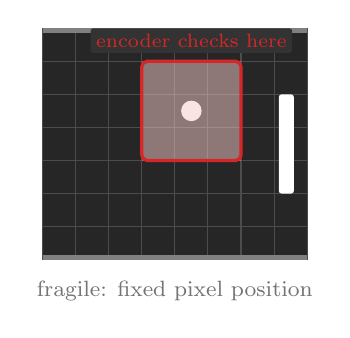
\begin{tikzpicture}[
    lbl/.style={font=\footnotesize, text=black!55},
]
\def\c{0.42}
\def\gw{8}
\def\gh{7}

% Dark game background
\fill[black!85] (0, 0) rectangle ({\gw*\c}, {\gh*\c});
% Subtle grid lines
\foreach \x in {0,...,8} {
    \draw[black!70] (\x*\c, 0) -- (\x*\c, {\gh*\c});
}
\foreach \y in {0,...,7} {
    \draw[black!70] (0, \y*\c) -- ({\gw*\c}, \y*\c);
}

% Top and bottom walls (Pong borders)
\fill[black!50] (0, 0) rectangle ({\gw*\c}, {0.15*\c});
\fill[black!50] (0, {6.85*\c}) rectangle ({\gw*\c}, {\gh*\c});

% Paddle (tall, thin, right side)
\fill[white!90, rounded corners=1pt]
    ({7*\c + 0.06}, {2*\c}) rectangle ({7.6*\c}, {5*\c});

% Ball
\fill[white] ({4.5*\c}, {4.5*\c}) circle (0.13);

% Spotlight: bright region at fixed position (cells 3-5, 3-5)
\fill[palB!25, opacity=0.5]
    ({3*\c}, {3*\c}) rectangle ({6*\c}, {6*\c});
\draw[palB, very thick, rounded corners=2pt]
    ({3*\c}, {3*\c}) rectangle ({6*\c}, {6*\c});

% Label on spotlight
\node[font=\scriptsize, text=palB, fill=black!80,
      inner sep=2pt, rounded corners=1pt, anchor=south]
    at ({4.5*\c}, {6*\c + 0.1})
    {encoder checks here};

% Verdict
\node[lbl] at ({4*\c}, {-0.4})
    {fragile: fixed pixel position};

\end{tikzpicture}
\subcaption{The encoder memorizes a fixed region. It works when
  the ball is there but fails if the image shifts.}
\label{fig:fragile-feature}
\end{subfigure}
\hfill
%% (b) Robust: object relationship
\begin{subfigure}[t]{0.47\textwidth}
\centering
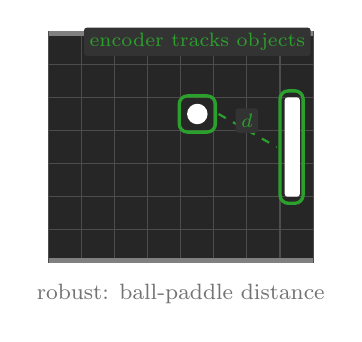
\begin{tikzpicture}[
    lbl/.style={font=\footnotesize, text=black!55},
]
\def\c{0.42}
\def\gw{8}
\def\gh{7}

% Dark game background
\fill[black!85] (0, 0) rectangle ({\gw*\c}, {\gh*\c});
% Subtle grid lines
\foreach \x in {0,...,8} {
    \draw[black!70] (\x*\c, 0) -- (\x*\c, {\gh*\c});
}
\foreach \y in {0,...,7} {
    \draw[black!70] (0, \y*\c) -- ({\gw*\c}, \y*\c);
}

% Top and bottom walls
\fill[black!50] (0, 0) rectangle ({\gw*\c}, {0.15*\c});
\fill[black!50] (0, {6.85*\c}) rectangle ({\gw*\c}, {\gh*\c});

% Paddle
\fill[white!90, rounded corners=1pt]
    ({7*\c + 0.06}, {2*\c}) rectangle ({7.6*\c}, {5*\c});

% Ball
\fill[white] ({4.5*\c}, {4.5*\c}) circle (0.13);

% Green highlight around ball
\draw[palC, very thick, rounded corners=3pt]
    ({4*\c - 0.02}, {4*\c - 0.02})
    rectangle ({5*\c + 0.02}, {5*\c + 0.02});

% Green highlight around paddle
\draw[palC, very thick, rounded corners=3pt]
    ({7*\c}, {1.8*\c})
    rectangle ({7.7*\c}, {5.2*\c});

% Distance line connecting ball to paddle
\draw[palC, thick, dashed]
    ({5*\c + 0.06}, {4.5*\c}) -- ({7*\c - 0.04}, {3.5*\c});
\node[font=\scriptsize, text=palC, fill=black!80,
      inner sep=2pt, rounded corners=1pt]
    at ({6*\c}, {4.3*\c}) {$d$};

% Label
\node[font=\scriptsize, text=palC, fill=black!80,
      inner sep=2pt, rounded corners=1pt, anchor=south]
    at ({4.5*\c}, {6*\c + 0.1})
    {encoder tracks objects};

% Verdict
\node[lbl] at ({4*\c}, {-0.4})
    {robust: ball-paddle distance};

\end{tikzpicture}
\subcaption{The encoder tracks the spatial relationship between
  ball and paddle -- a feature that survives any shift.}
\label{fig:robust-feature}
\end{subfigure}

\caption{Augmentation as regularization. (a)~Without augmentation,
  the encoder can rely on fixed pixel positions.
  (b)~Random shifts force it to learn object relationships.}
\label{fig:fragile-vs-robust}
\end{figure}
